\documentclass[UTF8]{ctexart}
%字体配置
%\documentclass[UTF8]{ctexreport}
%以上是报告版,可以添加章节
%这里可以书写注释

\usepackage{graphicx}
\usepackage{caption}
\usepackage{subfigure}
\usepackage{float}
\usepackage{cite}
\usepackage{url}
\usepackage{geometry}
\geometry{a4paper,scale=0.8}
%以上是使用图形包(傻瓜加入完事了)

\title{人机工学:个人调查报告}
\author{陈禹汀}
\date{2020/10/3}
%以上为文章属性设置
\begin{document}

\maketitle%自动制作标题
\newpage
\tableofcontents%生成目录
\newpage
%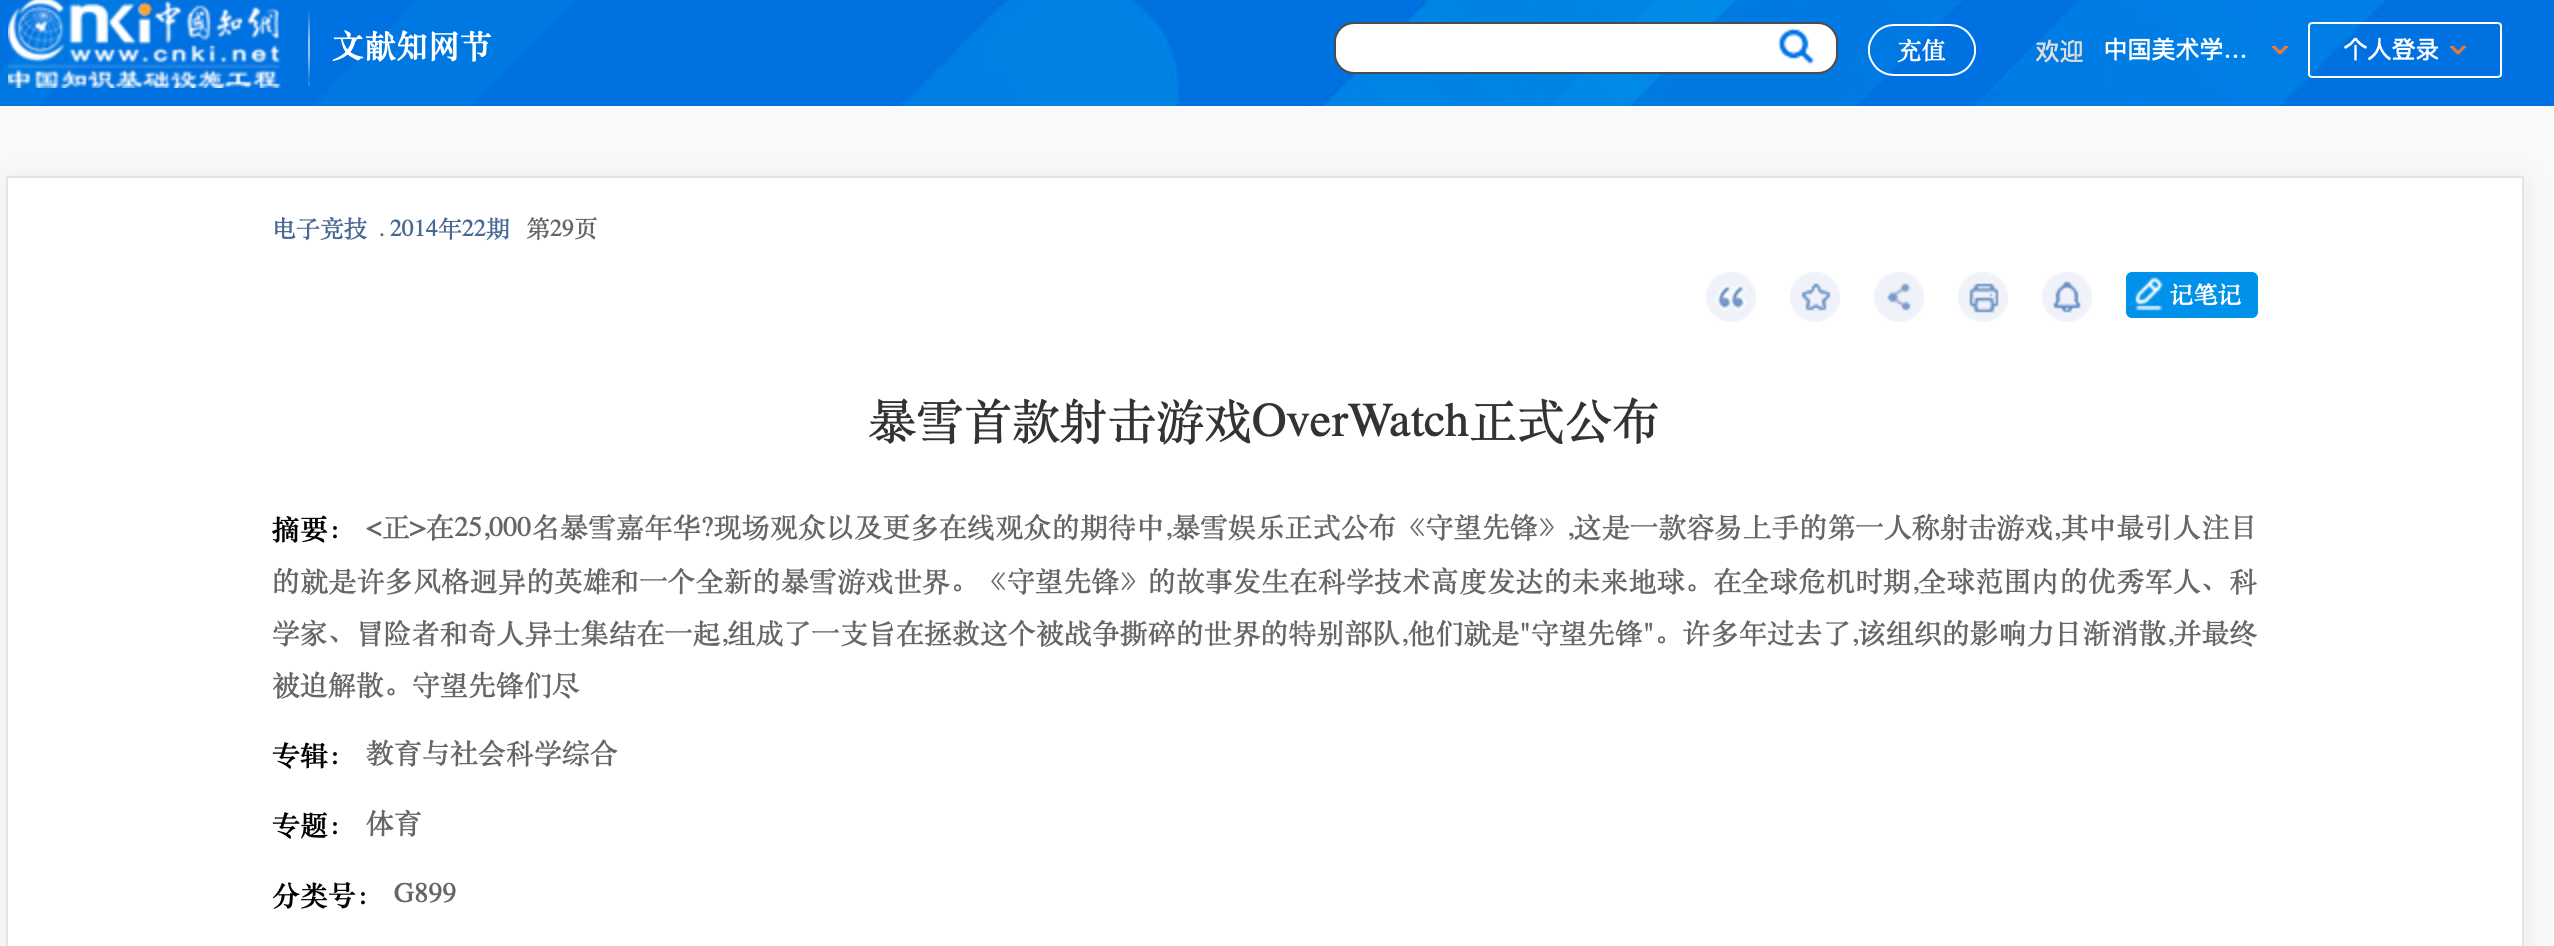
\includegraphics[width = .8\textwidth]{1.png}
%以上是插入图片
\section{个人调研}
    本次人机工学个人小作业调研的方向是电子竞技(主要游戏设备为个人电脑,主要游戏为《守望先锋》)中人体的动态。
\subsection{为什么是PC电子竞技?}
\paragraph{社会趋势}
    电子竞技正逐渐变成人类进行消遣行为的一种主要方式。"2020年突发疫情改变了人们文化消费的方式与内容,直接影响到生产端供给,以网络游戏、在线观影、短视频等为代表的数字文创产业成为文化消费的主力军." \cite{esports}
\paragraph{使用条件}
    虽然电子游戏的依附终端从比较难以携带的个人主机已经逐渐变到几乎成为“义肢”的智能手机。但是移动设备无法满足高强度的持续运行,以及高帧率高画质的性能,然而fps游戏往往需要这些性能来进行平滑的影像处理。 \cite{framerate}所以当前主要的大型电子竞技游戏平台依然是桌面端.
\subsection{为什么是《守望先锋》}
    守望先锋是一款结合fps和MOBA类风格的游戏,它像是《英雄联盟》、《DOTA2》这些MOBA类游戏,存在着高APM的操作 \cite{wiki:APM}。同时它也需要拥有《CS:GO》《战地(系列)》中准确瞄准能力。因而这是一款非常具有样本性的一款游戏。我们能够从它的操作行为模式中获取人与电子竞技类游戏之间的关系。
\subsection{DPI和EDPI是什么}
    DPI(Dots Per Inch),是鼠标移动一英寸在能够在屏幕上划过的像素的简称。例如当你的DPI设置为800时,若显示器分辨率为1080p,则你的手在桌上移动一英寸,鼠标将划过74\%的屏幕。你的DPI越高,你的鼠标在屏幕上的移动能力越灵敏。\cite{prosetting_dpi}
\paragraph{}
    EDPI(DPI * 游戏内灵敏度),也就是游戏中对于鼠标本身dpi的倍增,鼠标移动多少像素,游戏内就移动 鼠标移动像素*灵敏度(一般再乘以一个常数)个像素。这个值不宜太高,否则容易产生瞄准不到的像素,因而影响战斗时的打击精确度。
\newpage
\section{数据获取以及筛选}
\subsection{职业赛场数据}
    从不少的网站上可以仔细地查看到各大职业选手的鼠标和设备参数,我们能够从这些样本中获取不少信息。从prosettings网站上我们可以迅速地查阅到联赛选手和twitch主播的设置。 \cite{prosetting_edpi}在其中需要得到我们注重的是他们使用的鼠标、eDPI(灵敏度*鼠标DPI)以及与之成反比的360度转身鼠标转动距离。 \cite{prosetting_guide}这样我们能够统计出职业选手的普遍转动距离作为初步参考。
\begin{figure}[htbp]
    \centering
    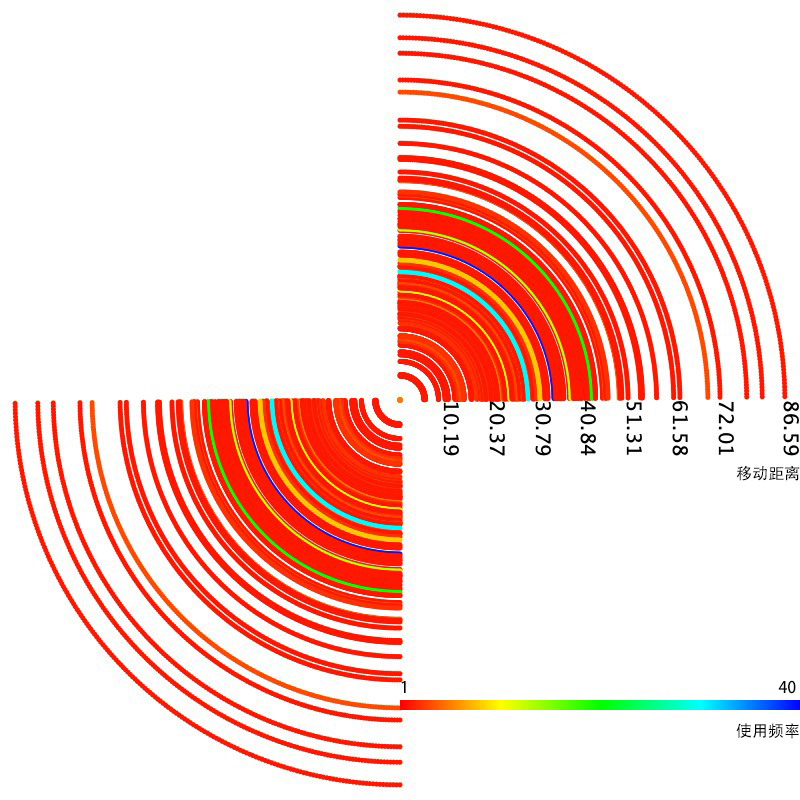
\includegraphics[width=0.45\textwidth]{out.jpg}
    \caption{职业选手360转身手臂移动距离相对距离与使用频率统计图}
    \centering
    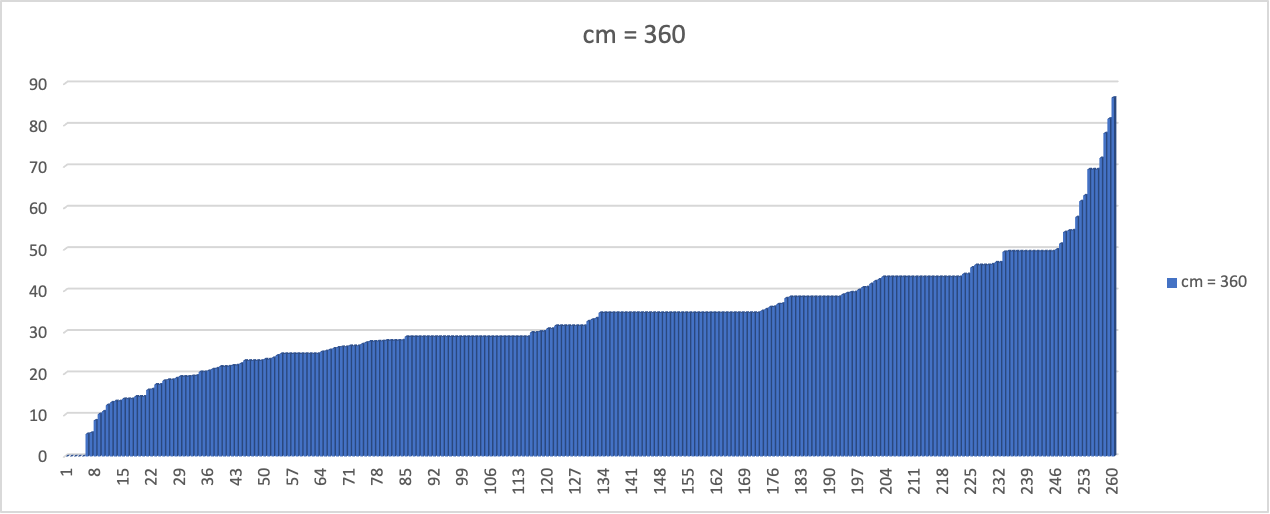
\includegraphics[width=1\textwidth]{proDataPoly.png}
    \caption{职业选手360转身手臂移动距离柱状图}
\end{figure}
\paragraph{分析}
    从图1中我们可以看到30.79-40.84范围内存在一根蓝色的线,而这根线代表着34.64cm/360度以及4000的eDPI,从数据表中可以看到有四十一位职业选手在使用这一设置,占据总选手数量的15.7\%(41/261)。而在柱状图中,两端虽然存在陡峭的曲线,但是中部的曲线增长率低且稳定。总体选手的eDPI/360度转身距离为4839/33.02cm,从平缓范围(eDPI 2400-13600)得到的eDPI/360度转身距离为4748/32.57。这个范围整体体现了专业选手们和高级玩家的设置,因而对于游戏来说往往是最佳设定范围。在本次调查中,将其设为最具有代表性的样本。
\subsection{个人使用数据整理}
    虽然本人算不上守望先锋高级玩家,但是竞技分数和排位尚可,也为自己的瞄准能力下了比较大的功夫。使用的dpi是800DPI*5的组合,也就是eDPI为4000。使用固定机位拍摄了一张进行正常游戏时的本人右手,使用opencv框架,通过模型获取近似手部区域,多次训练后获取总值较高的像素捕捉骨骼。标定骨架后计算手掌位置,统计输出桌面面积使用映射图。
\paragraph{}映射图如下。
    \begin{figure}[htbp]
        \centering
        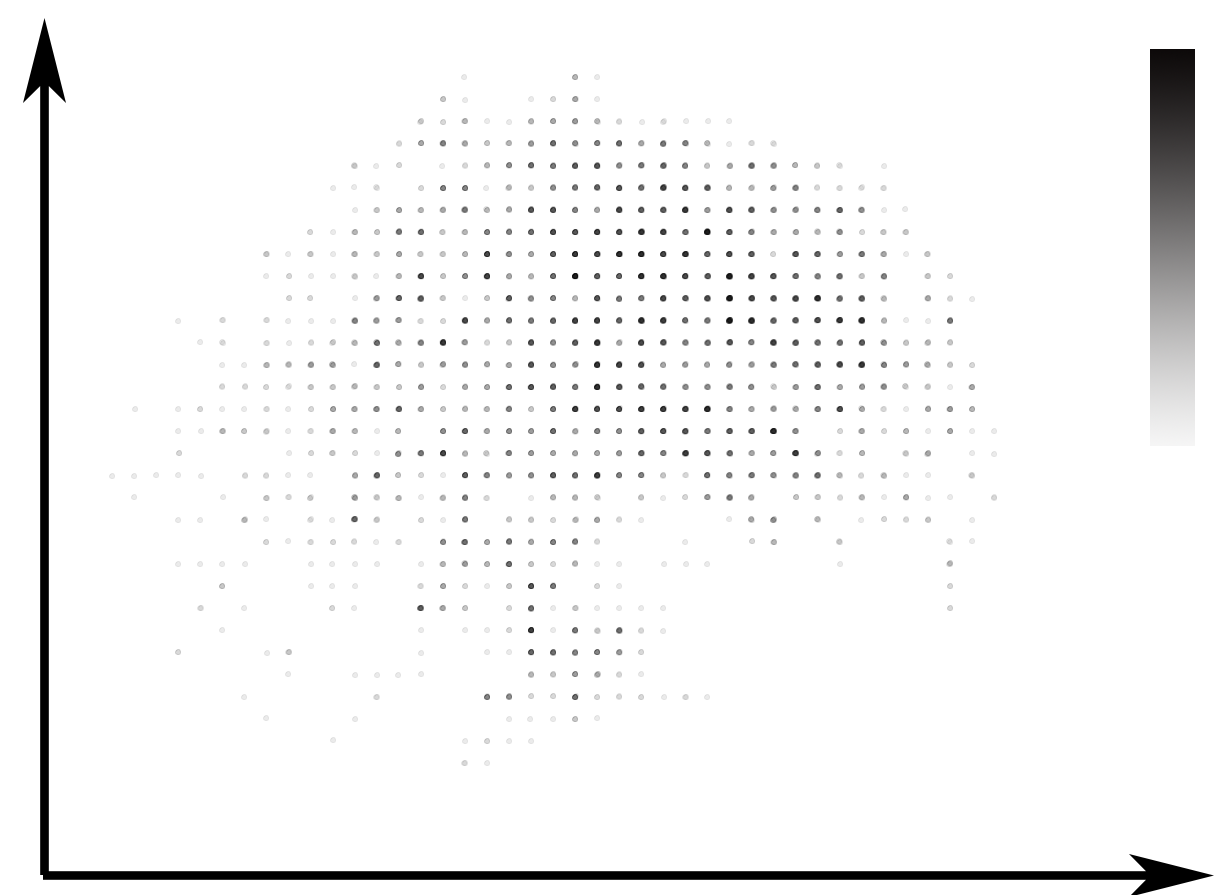
\includegraphics[width=0.45\textwidth]{point.png}
        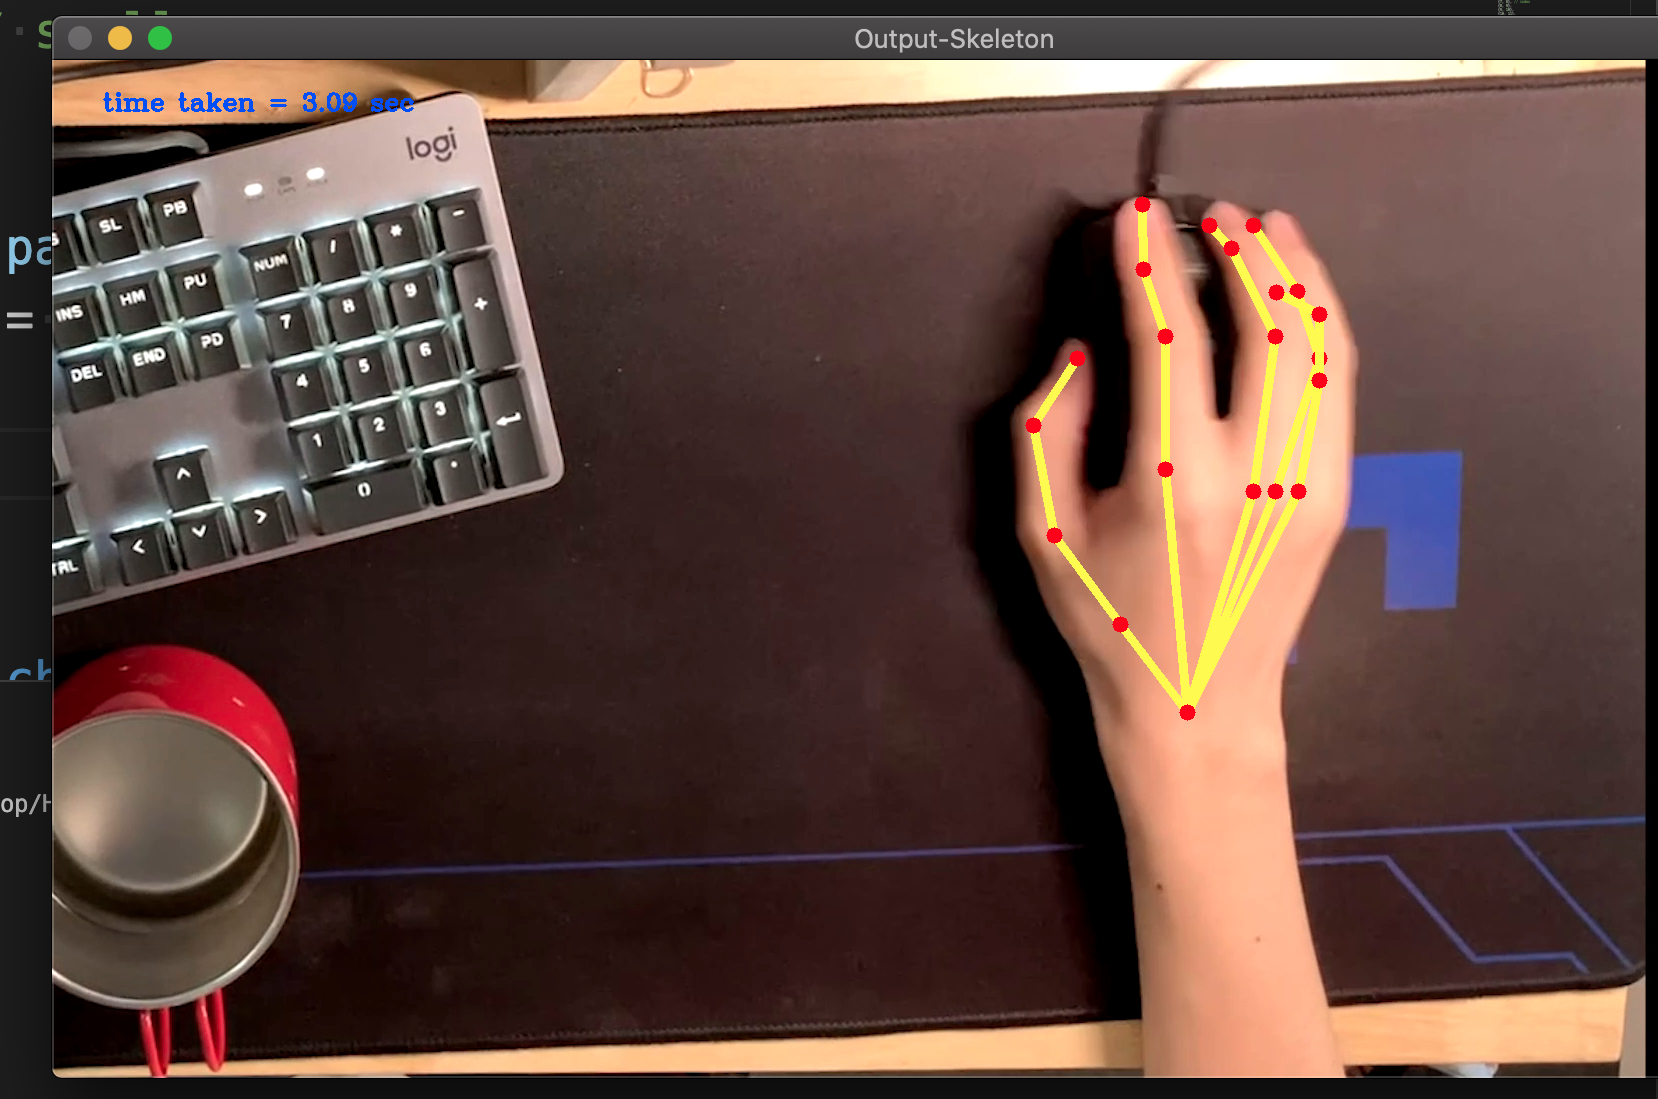
\includegraphics[width=0.45\textwidth]{test.png}
        \caption{桌面掠过面积及其频率散点图}
    \end{figure}
    \paragraph{分析}
    从图中可以看到,主要移动区域集中在中央部分,同时右下方存在一些缺口,这里是手腕所在的位置,因为寝室空间有限,其实使用的是手臂流,右手小臂和桌面存在30度到45度的角度。

\newpage
\section{运动模型}
%\subsection{鼠标到屏幕的动作映射}在标准情况下,水平灵敏度为30,垂直灵敏度为15,在灵敏度为5,DPI为800的情况下,横向移动34.64厘米能够使镜头横向旋转360度,纵向移动同样距离能够在竖直方向使镜头旋转180度。
\subsection{鼠标到屏幕的动作映射}像守望先锋等游戏能够定量转换鼠标硬件移动量到摄像机角度。在标准情况下,水平灵敏度为30,垂直灵敏度为15,在eDPI为4000的情况下,横向移动34.64厘米能使镜头横向旋转360度,纵向移动相同厘米数能使镜头纵向旋转180度。
\newline
以下是经过测算的移动距离和dpi的关系以及dpi与鼠标垫有效使用面积关系。
\begin{figure}[htbp]
    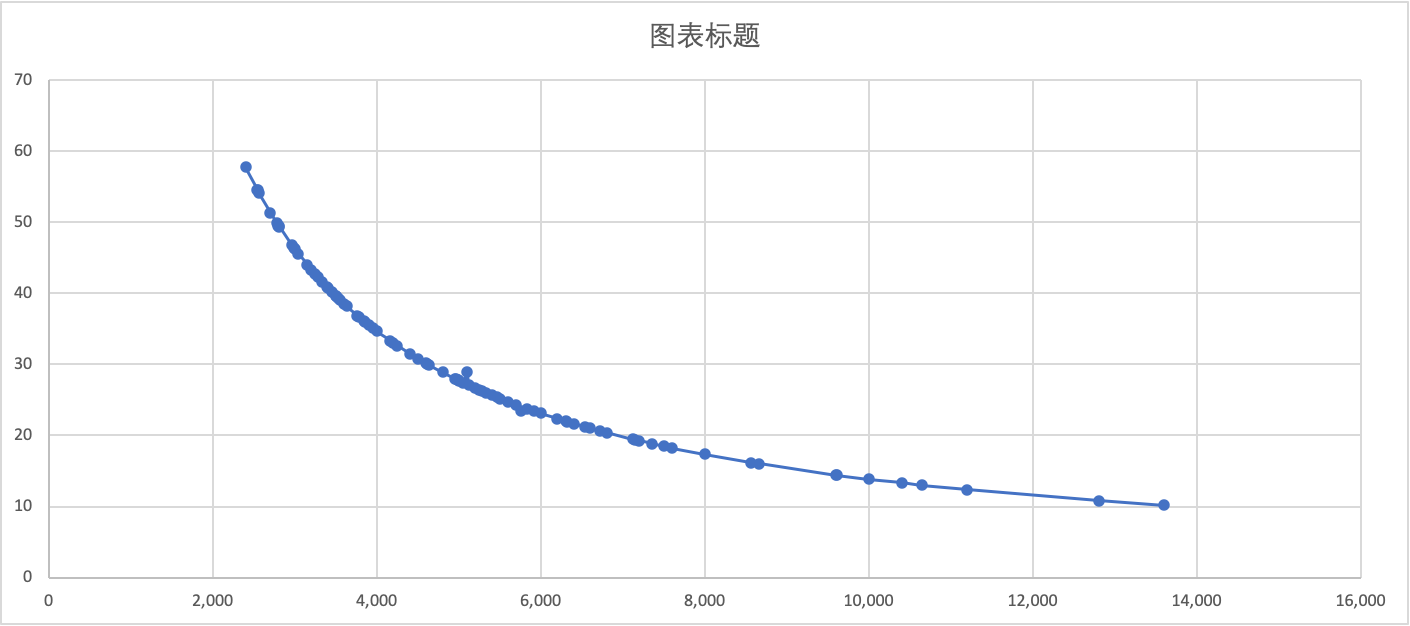
\includegraphics[width=0.45\textwidth]{calculate.png}
    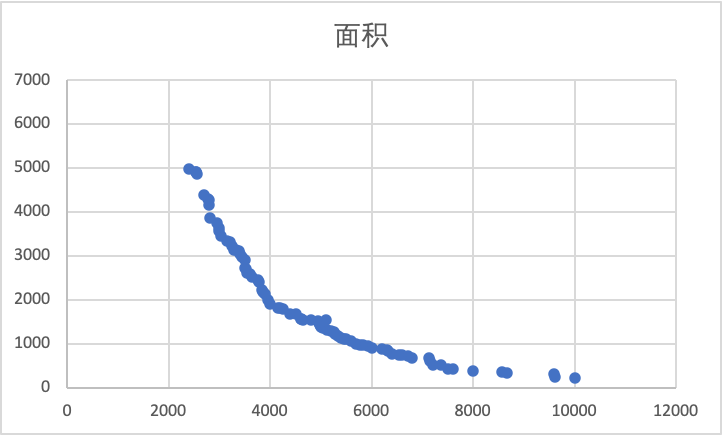
\includegraphics[width=0.45\textwidth]{field.png}
\end{figure}
\paragraph{}如果使用以上数据就能够推算出鼠标在桌面上的目标运动距离。


\subsection{鼠标-手腕-手臂模型}
    %鼠标重量与鼠标移动范围,右侧面标注小手臂和桌面之间的尺寸,顶面标注手部移动的范围。
    \begin{figure}[htbp]
        \centering
        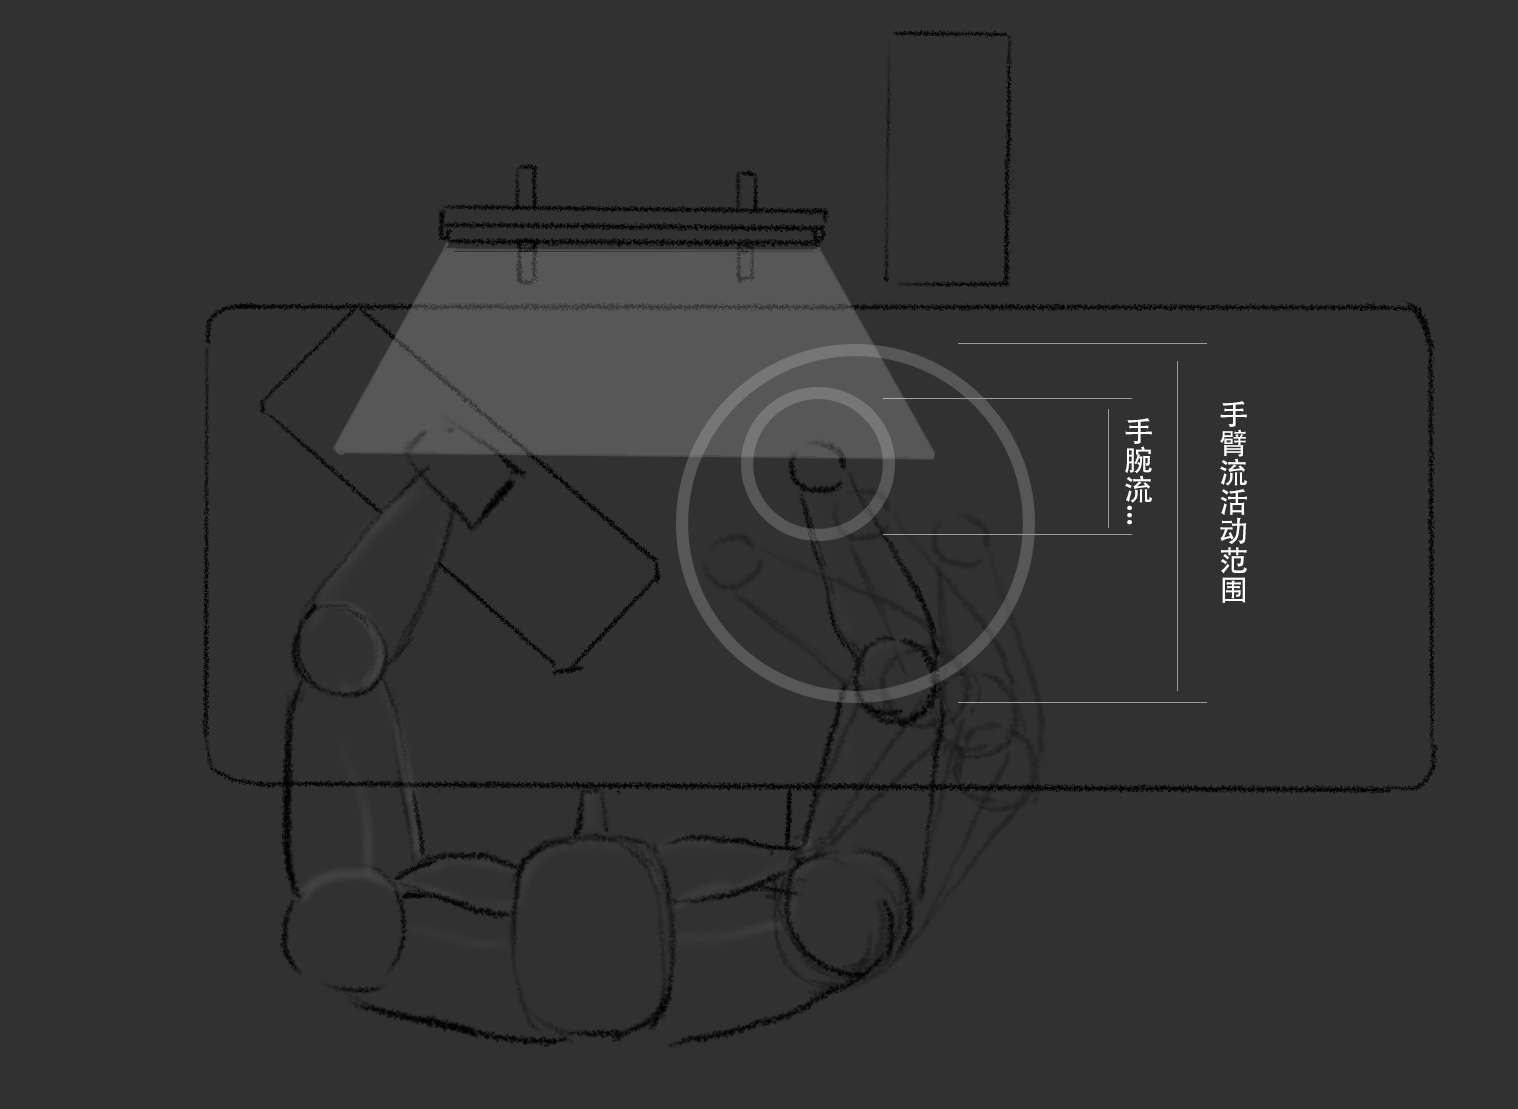
\includegraphics[width=0.45\textwidth]{desktop.png}
    \end{figure}
    \paragraph{两大瞄准方式:手臂/手腕}
    \paragraph{}手腕流:手腕为轴心转动,尺骨大部分(约四分之三)悬空,小范围内操控舒适,准星微操作精准。大范围转动视角受限,为了方便转头通常会将鼠标速度设置的较高。

    \paragraph{}
    以edpi高达24400的纽约九霄天擎队队员Haksal为例子,作为知名的微操选手,他的理论活动范围为5.68cm*5.68cm*2,大约是一个正常人类掌心的大小。因而他是个在游戏内转身非常灵活的选手。
    \paragraph{}
    手臂流:肘部为轴心转动,尺骨大部分搁置在桌面上。操控范围大约为整个小臂移动的范围,需要更大的鼠标垫。鼠标速度较慢,通常以大范围的手臂移动弥补,操控更加稳定细腻。
    \paragraph{}
    以守望先锋第一赛季常规赛MVP“JJonak”为例,他的edpi为2000,横向360转身长度为69.27cm,因为鼠标垫大小的限制,往往他只能做出两次180度转身(即将鼠标拖动34.635cm后提起鼠标,将其重置在鼠标垫一侧之后再次拖动)。
    \cite{zhihu_liupai}
\subsection{其他身体部位的移动范围}
    %侧面线稿,标注桌面和肩膀相对高度,桌面与胸口相对高度
    \begin{figure}[htbp]
        \centering
        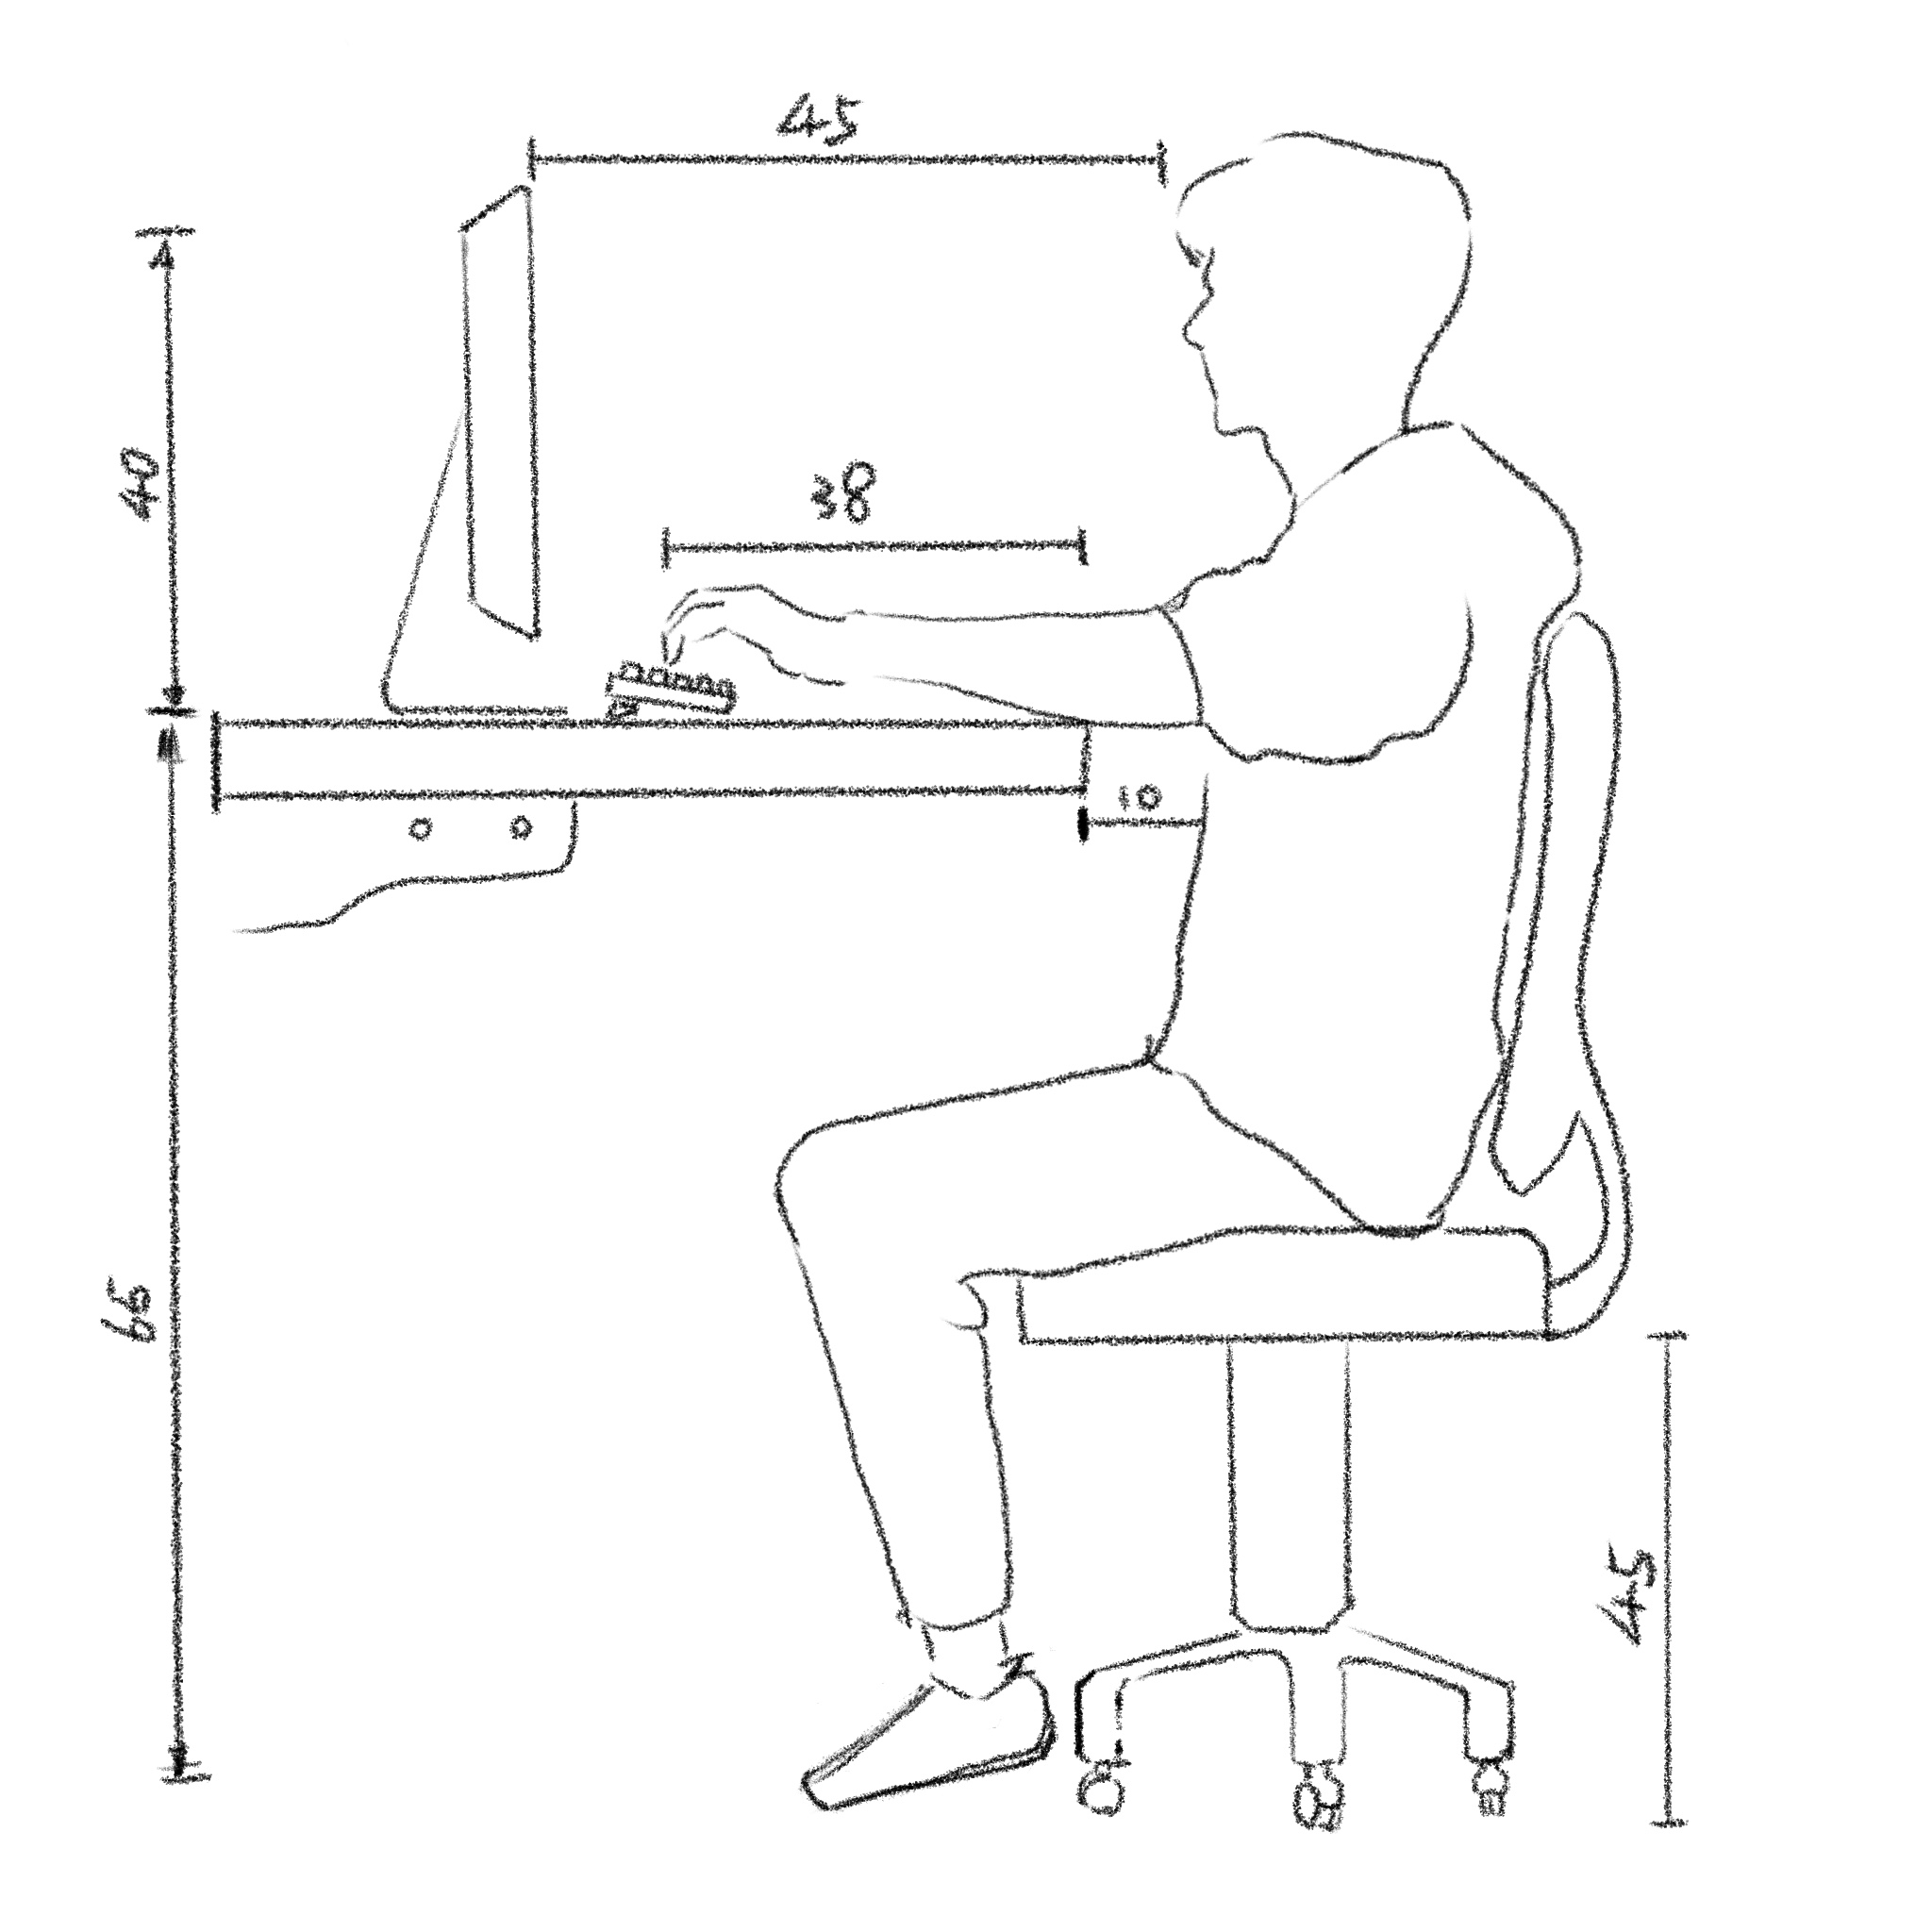
\includegraphics[width=0.45\textwidth]{desktop.jpg}
    \end{figure}
    \paragraph{分析}
    电竞产业的总体身体坐姿需求可能和普通办公差距并不大,重点是保持人体脊柱受力平衡同时保持小臂能够较为舒适地安放在桌面上,即保持桌面至肩膀的距离为大臂的长度。将桌面边缘靠的离胸口较近,这样能够提供一个较为自由的甩动距离。同时注重于保持显示器和头部成舒适角度,一般将视觉中心设置为抬头时眼镜的水平线上。


\section{痛点分析}
\paragraph{大体职业氛围}
%职业病例距离/病理跟踪
\paragraph{fps职业氛围}
%手腕预期寿命,状态保持时间

\section{改进}

\newpage
\bibliographystyle{ieeetr}
\bibliography{myref}    

\end{document}

